\subsection{Ejercicio 5}

Para el ejercicio 5 se nos pidi\'o dise\~nar e implementar un algoritmo de \textit{scheduling} basado en la publicaci\'on de Waldspurger, C.A. y Weihl, W.E llamada \textit{Lottery scheduling: Flexible proportional-share resource management}.

\subsubsection{Introducci\'on}

El algoritmo de \textit{Lottery scheduling} establece un sistema de prioridad para la obtenci\'on de los recursos del sistema por parte de los procesos, basado en \textit{tickets} de loter\'ia. Cada proceso es due\~no de una determinada cantidad de tickets. En cada elecci\'on de un nuevo proceso a correr por parte del scheduler, se realiza una loter\'ia entre todos los tickets del sistema, eligi\'endose uno al azar. El pr\'oximo proceso a correr es el due\~no del ticket ganador, quien se ejecutar\'a hasta la finalizaci\'on del \textit{quantum}, y el proceso se repite.

\subsubsection{Asignación de recursos}

La distribuci\'ion de los tickets y posterior elecci\'on aleatoria de uno de ellos establece un sistema de prioridades probabil\'istico basado en la cantidad de tickets que posee cada proceso. Por ejemplo, sean A y B dos procesos en un sistema de 100 tickets, teniendo A 75 tickets y B 25, se esperar\'ia que el proceso A posea el 75\% de los recursos del sistema y B el 25\%. Dado el car\'acter no determin\'istico del algoritmo, no es posible confirmar que esto suceda para cualquier ejecuci\'on de las tareas. Pero la probabilidad de que esto suceda aumenta conforme a la cantidad de ejecuciones, como se mostrar\'a en la secci\'on de experimentaci\'on. Dada que la asignaci\'on de recursos esperada es proporcional a la cantidad de tickets que posee cada proceso, decimos que \textit{Lottery Scheduling} es probabil\'isticamente justo.

Los tickets \textit{encapsulan} la gesti\'on de la asignaci\'on de los recursos del sistema, ya que cuantifican la posesi\'on de \'estos por parte de los procesos independientemente de los detalles de la m\'aquina. Dado que en un determinado sistema puede haber diversos recursos heterog\'eneos, realizan una abstracci\'on uniforme de \'estos ya que la probabilidad de asignaci\'on de cualquiera de ellos a un proceso se representa homog\'eneamente a trav\'es de tickets. 

Esta representaci\'on facilita tambi\'en los cambios de prioridad entre los determinados procesos.

\textit{Nota: Dado que el \'unico recurso de sistema que se gestiona en nuestra implementaci\'on del scheduler es el tiempo de CPU, de ahora en m\'as solo nos referiremos a \'este.}

\subsubsection{Optimizaciones}

El concepto b\'asico de \textit{Lottery Scheduling} puede mejorarse considerablemente mediante la implementaci\'on de algunos mecanismos, explicados a continuaci\'on:

\begin{itemize}

\item \textit{Transferencia de tickets:} cuando un proceso est\'a bloqueado esperando la respuesta de otro proceso, puede transferir sus tickets a \'este, causando una mejora de perfomance ya que va a tener m\'as probabilidad de obtener el CPU, agilizando la respuesta. Cuando el primer proceso recibe la respuesta, le son devueltos sus tickets. De esta forma se resuelve el problema de la proridad inversa, de una manera similar a herencia de prioridades.

\item \textit{Tickets compensatorios:} los procesos que se bloquean en espera de una respuesta externa y no consumen el total de su quantum terminan obteniendo menos tiempo de CPU del que les corresponde, rompiendo el modelo de asignaci\'on en cuanto a la probabilidad. La forma de solucionar esto es la asignaci\'on de tickets compensatorios a estos procesos. De esta forma cuando un proceso utiliza una fraci\'on de su quantum, recibir\'a tickets aumentando su probabilidad de ser elegido para el pr\'oximo quantum.

\item \textit{Inflaci\'on de tickets:} cuando un proceso sabe que debe ejecutar una secci\'on cr\'itica y considera que va a necesitar m\'as tiempo de CPU, puede aumentar su n\'umero de tickets. Esta es una forma simple y eficiente de reflejar esa necesidad en el sistema, y no es necesario comunicarse con los otros procesos. Cabe aclarar que, este m\'etodo s\'olo es utilizable en un sistema donde los procesos ejecutan de forma cooperativa. 

\end{itemize}

\subsubsection{Resumen: Ventajas de Lottery Scheduling}

\begin{itemize}

\item Implementaci\'on sencilla y eficiente.

\item Provee encapsulaci\'on abstracta, relativa y uniforme de los recursos.

\item El usuario puede realizar la distribuci\'on de tickets entre sus procesos, estableciendo prioridades.

\item Realiza una distribuci\'on de los procesos probabil\'isticamente justa. 

\item La randomizaci\'on es una elecci\'on r\'apida, f\'acil de implementar, independiente de las anteriores y libre de peores casos.

\item Se puede especificar qu\'e porcentaje de procesador le corresponde a cada proceso.

\item Se resuelve el problema de la inanici\'on. Siempre y cuando un proceso tenga al menos un ticket, tiene una probabilidad no nula de ser elegido.

\item Gracias al sistema de \textit{currency}, puede implementarse un sistema modular de gesti\'on de recursos.

\item Mediante el concepto de \textit{ticket transfer}, un proceso bloqueado esperando respuesta de otro proceso puede transferir sus tickets a \'este, solucionando el problema de la prioridad inversa.


 \end{itemize}

\subsubsection{Posibles desventajas}

\begin{itemize}

\item Si bien la naturaleza aleatoria del algoritmo tiene ventajas, posee como desventaja nunca poder asegurar determin\'isticamente un resultado.

\item La asignaci\'on de los tickets a los procesos es un problema en s\'i mismo no abarcado por los autores. El comportamiento de un sistema va a depender fuertemente de la distribuci\'on de los tickets.

\end{itemize}

\subsubsection{Detalles de la implementaci\'on}

A continuaci\'on expondremos los detalles de nuestra implementaci\'on particular de \textit{Lottery Scheduling}. Dado que la probabilidad de ser asignado el CPU para cada proceso depende solamente de la cantidad de tickets que posea, y no de cu\'ales sean \'estos, no diferenciaremos entre tickets, s\'olo nos va a interesar la cantidad de tickets que posea cada proceso.


\vspace{2mm}

El sistema comienza con una cantidad de 100 tickets que son distribuidos equitativamente entre todos los procesos al comenzar, para garantizar la misma probabilidad a todos. Nuestra elecci\'on de 100 como n\'umero de tickets inicial se debe a que el c\'alculo de la probabilidad de cada proceso en base a su n\'umero de tickes es simple e inmediato, y nos provee de presici\'on suficiente. Es importante tambi\'en notar que en la experimentaci\'on, no habr\'a m\'as de 100 tareas ejecut\'andose en un mismo experimento. De todas formas la soluci\'on a esto no es m\'as que cambiar la variable por un n\'umero mayor, por ejemplo 1000.

\vspace{2mm}

La estructura de datos elegida para almacenar las tareas y su cantidad de tickets correspondiente es una lista de pares$<pid, \#tickets>$. La forma de conocer si una tarea est\'a lista para ser ejecutada es otro diccionario$<pid, bool>$, que indica, para el valor verdadero que la tarea se encuentra en estado $ready$, y para el valor falso que se encuentra en estado $block$ o $exit$.

\vspace{2mm}

\textbf{Estructuras de datos:}

\begin{itemize}

\item $int$ quantum: almacena el valor de quantum pasado por par\'ametro.

\item $int$ cantTicks: almacena la cantidad de ticks de reloj que pasaron desde el \'ultimo cambio de tarea.

\item $int$ semilla: almacena la semilla pseudoaleatoria

\item $list<pid, cantTickets>$ tareasYTickets: lista que almacena las tareas del sistema y para cada una, la cantidad de tickets que posee

\item $map<tarea, bool>$ bloqueadasTerminadas: diccionario que indica para cada tarea si se encuentra lista para ejecutar.

\end{itemize}


\vspace{2mm}

Nuestra clase scheduler recibe como par\'ametros el quantum y la semilla pseudoaleatorioa. \textit{SchedLottery} hereda de la clase \textit{SchedBase},y por lo tanto implementa las funciones \textit{load()}, \textit{unblock()} y \textit{tick()}, adem\'as cuenta con:


\vspace{2mm}

\textbf{Funciones}

\begin{itemize}

\item $load():$ carga una nueva tarea que llega al scheduler, agreg\'andola a ambos diccionarios, y repartiendo nuevamente los tickets entre todos los procesos de forma equitativa.

\item $unblock(): $ desbloquea una tarea, actualizando su valor en el diccionario bloqueadasTerminadas.

\item $tick(): $ se ejecuta en cada tick del reloj, incrementando en $1$ la cantidad de ticks de la tarea actual. En caso de que se agote el quantum de \'esta, se desaloja y se llama a loter\'ia. Si la tarea se bloque\'o se actualiza en el diccionario bloqueadasTerminadas y se llama a loter\'ia. Si la tarea En caso de que no queden m\'as tareas a ejecutar, finaliza la ejecuci\'on pasando a la tarea IDLE\_TASK.
\item $loteria(): $ se realiza la loter\'ia, eligiendo la nueva tarea a ejecutar. Se explica a continuaci\'on.

\end{itemize}

\subsubsection{Loter\'ia}

Como mencionado anteriormente, nuestra implementaci\'on no diferencia entre tickets, solamente se tiene en cuenta la cantidad de ellos que cada proceso posee. La forma de elegir al ticket ganador, es elegir un n\'umero pseudoaleatorio entre 0 y la cantidad total de tickets. Acto seguido, se recorre la lista de tareas, y se realiza una suma parcial de la cantidad de tickets de las tareas recorridas. Se itera por las tareas, mientras la suma parcial sea menor al n\'umero ganador. La tarea ganadora va a ser aquella en la cual la iteraci\'on termine, es decir, la primera tal que la suma parcial $+$ la cantidad de tickets de la tarea ganadora supera el numero pseudoaleatorio elegido.

\begin{center}
    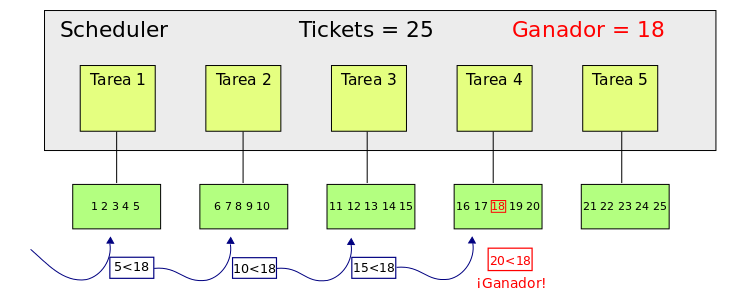
\includegraphics[scale=0.6]{./Graficos/loteria.png}
\end{center}

Dado que los tickets poseen todos el mismo valor de probabilidad, y son uniformes, de esta forma se produce una numeraci\'on autom\'atica en cada loter\'ia realizada, donde si cada tarea posee $k$ tickets, entonces sus tickets son los del intervalo de n\'umeros enteros [$sumaParcial$ .. $sumaParcial + k$].Consideramos correcta esta implementaci\'on, ya que es an\'aloga a enlistar los tickets en un vector, y en lugar de elegir el ticket de acuerdo a su n\'umero como en una loter\'ia, se eligen de acuerdo a su posici\'on en el vector (lo cual es equivalente, ya que los tickets son todos distintos y equiprobables).

\vspace{2mm}

Como por cuestiones de perfomance NO BLOQUEAMOS (NO SE)

\subsubsection{Optimizaciones}

Desde el punto de vista de performance, realizamos la optimizaci\'on sugerida por los autores para agilizar la b\'usqueda de la tarea ganadora. Esta b\'usqueda se realiza en tiempo lineal sobre la lista de tareas, buscando a la tarea due\~na del ticket ganador. Si ordenamos la lista seg\'un la cantidad de tickets de cada tarea de forma decreciente puede obtenerse una mejora de performance, ya que aquellas tareas con mayor cantidad de tickets tienen m\'as probabilidad de poseer el ticket ganador. Dado que es necesario ordenar la lista, lo realizaremos s\'olo en caso de que cambie la distribuci\'on de tickets, por ejemplo, cuando se carga una nueva tarea o cuando termina. 

\vspace{2mm}

Desde el punto de vista algor\'itmico, los autores propon\'ian diversas modificaciones que refinaban el modelo de \textit{Lottery Scheduling}. El scheduler posee la optimizaci\'on de \textbf{tickets compensatorios} previamente descripta.

\vspace{2mm}

Cuando se bloquea una tarea, nuestra implementaci\'on de los tickets compensatorios calcula la fracci\'on $f$ de quantum que \'esta utiliz\'o. Acto seguido multiplica la cantidad de tickets de la tarea por $1/f$. Como cada tarea posee la misma cantidad de tickets, ahora la tarea en cuesti\'on tiene $1/f$ m\'as probabilidad de salir que las dem\'as, siendo efectivamente compensada en la elecci\'on del siguiente quantum. HACER EXPLICACION

Las dem\'as optimizaciones no fueron consideradas por las siguientes razones:

\begin{itemize}

\item \textbf{Transferencias de tickets:} las tareas simuladas son independientes, y no se bloquean esperando una respuesta de otra tarea.

\item \textbf{Inflaci\'on de tickets:} las tareas simuladas ejecutan instrucciones fijas, en ning\'un momento ejecutan alguna secci\'on cr\'itica en la cual requieran m\'as tiempo de CPU. 

\end{itemize}

